\newpage
\section{PROBLEM II. [Evacuation Planning In Disaster Responses]}
	\subsection{Summary of the Problem}

	\qquad This problem is the planning of evacuation in case of the happening of a disaster presented by Li Wang (2020). The model used for this problem combines pre-event emergency evacuation plan with scenario-based evacuation plan for affected people after an event. Therefore, it consists of two stages with first-stage decisions being made in the advance of realization of uncertainty, and second-stage plans, which is time-dependent, being made after the realization of stochastic travel times (cost) and capacities.

	\qquad Similar to PROBLEM 1, the problem of interest is to solve the robust plan in the first stage with the result of the adaptive plan in the second stage. Therefore, Li Wang has formaluted a 2-stage model in time-dependent and random environment as below:

	\begin{figure}[htbp]
		\centering
		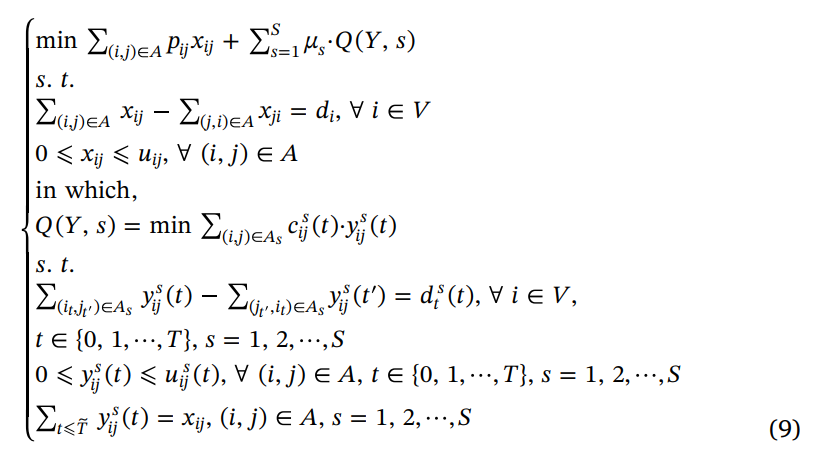
\includegraphics[width=0.8\textwidth]{graphics/liwang_model_1.png}
	\end{figure}

	\qquad This model is a time-dependent and stochastic two-stage evacuation planning model. Because it has a limited number of scenarios, the above model can be combined into the following single-stage stochastic model:

	\begin{figure}[htbp]
		\centering
		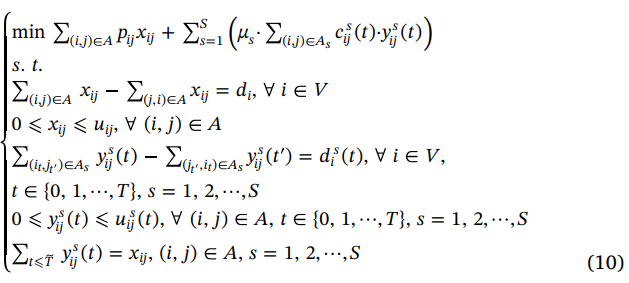
\includegraphics[width=0.8\textwidth]{graphics/liwang_model_2.png}
	\end{figure}

	\qquad This is essentially an integer programming model which contains two types of decision variables and a complex constraint. Therefore, we use Lagrangian relaxation to decompose it into two subproblems. The algorithm 1 proposed in the paper hold our interests, hence an implementation and efficiency verification are presented below.

	\subsection{Effectiveness verification}

	\qquad We used Primal Dual algorithm - and Successive Shortest Path algorithm to find the solution for the min cost max flow problem proposed in Li Wang’s research. The tables below illustrate the average runtime which obtained through executing 10 individual tests for each graph with number of vertices from 2 to 10, so there are 100 testcases.
	
	\begin{figure}[htbp]
		\centering
		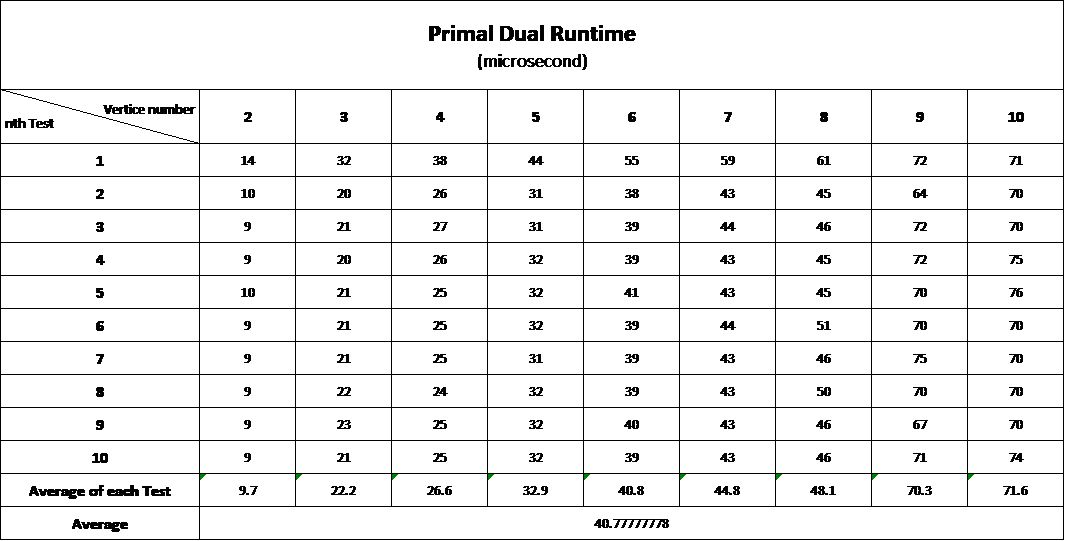
\includegraphics[width=0.8\textwidth]{graphics/table1.png}
		\caption{Runtime of Primal Dual algorithm}
	\end{figure}

	An $O(Fnmlogn)$ implementation of the successive shortest path algorithm ($F$ is the maximum possible flow, $n$ is the number of vertices, $m$ is the number of edges). Uses Bellman-Ford derivative to compute the initial potentials and uses Dijkstra to find the shortest paths. Note: The algorithm will fail if there is a negative cost cycle [4].

	\begin{figure}[htbp]
		\centering
		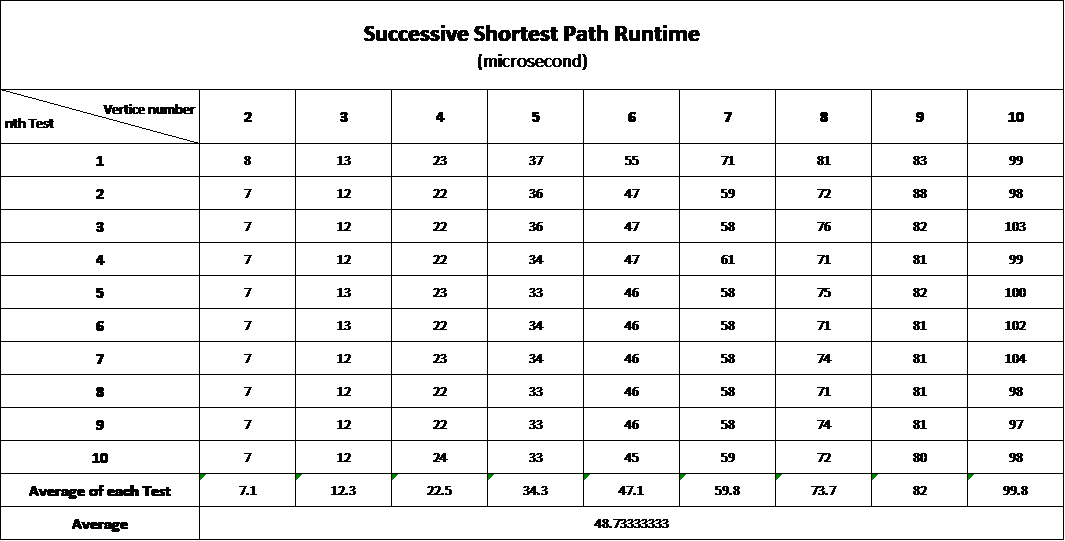
\includegraphics[width=0.8\textwidth]{graphics/table2.png}
		\caption{Runtime of Successive Shortest Path algorithm}
	\end{figure}

	\qquad An $O(Fn2m)$ implementation of a variation of the Primal-Dual algorithm (F is the maximum possible flow, n is the number of vertices, m is the number of edges). Usually performs much better in practice. Performs $O(F)$ augmenting loops in which it uses a modification of the Bellman-Ford algorithm to compute the potential for each node and uses a modification of the Dinic’s algorithm to saturate paths with cost equal to the potential of the sink node. Note: The algorithm will fail if there is a negative cost cycle [3].

	\qquad It is apparent that, the successive shortest path algorithm presents a relatively slower execution time than Primal Dual (about 0.8 microseconds). However, with a small number of vertices, specifically in a spectrum from 2 to 4, successive shortest path definitely superior to Primal Dual in terms of average runtime.
	